% Discuss the PEAR work and how it is relevant

\chapter{Physically Enhanced Authentication Ring}
\label{chapter:pear}

\section{Overview}
One problem that is present when using computers is that users typically are not aware of the security of the system
they are using. For instance, an attacker could have installed a key logger on a user's system to harvest every username
and password they have. Even with the best security systems on the machine in place, if the attacker is able to capture
a user's keystrokes, the other security is moot. 

PEAR, or Physically Enhanced Authentication Ring, was designed to counteract this key logger threat to a system. In addition
to defending against keyloggers specifically, it increases security in general because it is the second part of a "two factor
authentication" system. It also is a physical system, specifically a peripheral physical system, since it incorporates its
own processing and interacts with the user's normal computer system. Thirdly, the PEAR system incorporates a PUF device,
so it is a good example of when PUF technology is useful.

From a high level perspective, a PEAR device is a device consisting of a PUF, a keypad, and some supporting circuitry. When
a user wishes to log on to a given service, rather than using the keyboard for a password, he enters a 4 digit PIN on the PEAR
device. The PEAR device then executes the PUF and then initiates a zero-knowledge proof of knowledge with the service
provider. Note that no sensitive data is actually input to the PC, which potentially has a keylogger. Any data that the PC
is requested to ferry between the PEAR device and the service provider is encrypted, so recording this data does not reveal
any information.

The system works by having every service provider associated with an ID number of some kind. Each user of the service will
also have an ID number associated with it. This allows both parties to identify themselves to each other.

\section{Protocol Details}
The PEAR system consists of two parts, an enrollment step initially and then an authentication step.
Table~\ref{tab:pearprotocol} presents a formalized description of the protocols, while Figure~\ref{fig:pearauthentication}
and Figure~\ref{fig:pearenrollment} give graphical representations that occur.

An interesting point to note is that during the enrollment stage, an "out of band" communication is required to deliver
the combination of the service provider's ID, the user's corresponding ID for that service, and a nonce value. This could
be done by installing these values on the hardware device before it is given to an end user. For instance, if PEAR was being
used with a bank, the bank might install these values before mailing the device to the user.

\begin{figure}[!ht]
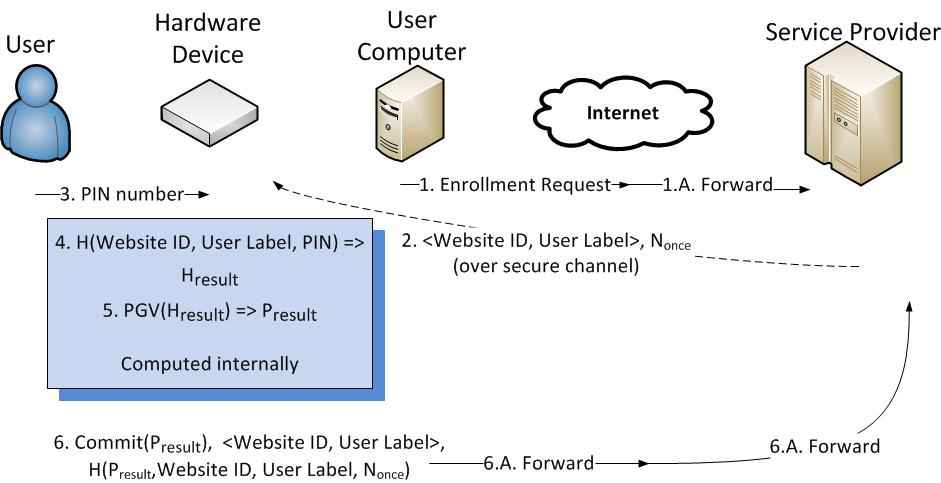
\includegraphics[width=500px]{images/enrollment.jpg}
\label{fig:pearenrollment}
\caption{The enrollment stage of PEAR}
\end{figure}
\FloatBarrier

\begin{figure}[!ht]
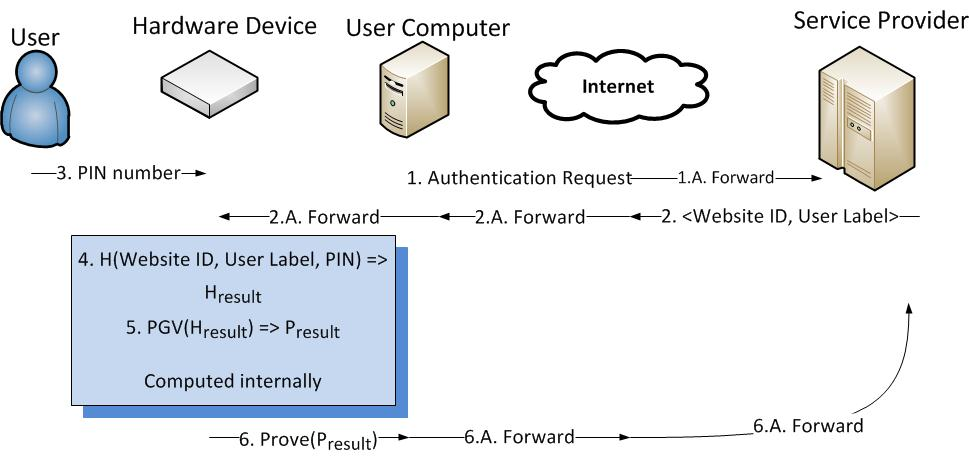
\includegraphics[width=500px]{images/auth.jpg}
\label{fig:pearauthentication}
\caption{The authentication stage of PEAR}
\end{figure}
\FloatBarrier

\begin{table}[!ht]
\label{tab:pearprotocol}
\caption{More formalized version of the PEAR protocols}
\noindent\makebox[\textwidth]{%
\begin{tabular}{|l|}
\hline
{\sf Enroll}($U$) - Device $T$ (using input data from user $U$) computes a commitment and enrolls the results with $S$. \\
\hline
- $C$ requests enrollment from $S$ \\
- $S$ sends the tuple $<$Label, ID$>$ and nonce $N$ to $T$ over a secure channel \\
- $U$ sends PIN to $T$ \\
- $T$ computes {\sf H}(ID, Label, PIN) as $H_{result}$ \\
- $T$ executes {\sf PGV}($H_{result}$) as $P_{result}$ \\
- $T$ sends {\sf Commit}($P_{result}$), $<$Label, ID$>$, {\sf H}({\sf Commit}($P_{result}$),Label,ID,$N$) to $S$, via $C$ \\
\hline
\hline
{\sf Authenticate}($U$) - Device $T$ (using input data from user $U$) authenticates itself as a registered user of $S$. \\
\hline
- $C$ initiates the authentication request from $S$ \\
- $S$ sends the tuple $<$Label, ID$>$ and {\sf Chal}($P_{result}$) to $T$ \\
- $U$ sends PIN to $T$ \\
- $T$ computes {\sf H}(ID, Label, PIN) as $H_{result}$ \\
- $T$ executes {\sf PGV}($H_{result}$) as $P_{result}$ \\
- $T$ responds with {\sf Prove}($P_{result}$), which $C$ forwards to $S$ \\
\hline
\end{tabular}
}
\end{table}
\FloatBarrier

\section{Security Considerations}

\section{Implementation}
From a high level view, Figure~\ref{fig:peararchitecture} describes the architecture of a PEAR enabled device.

\begin{figure}[!ht]
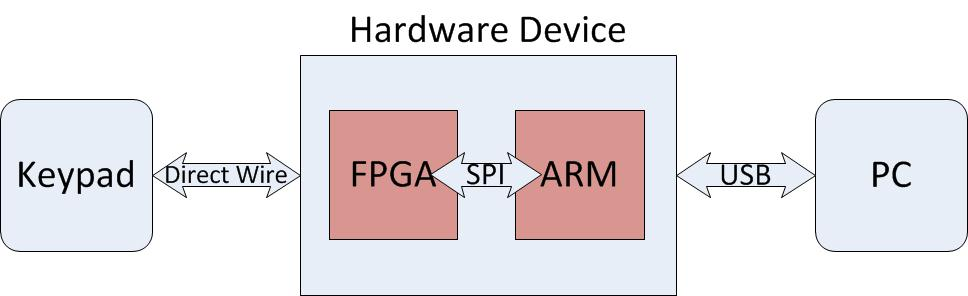
\includegraphics[width=500px]{images/pearimpl.jpg}
\label{fig:peararchitecturet}
\caption{Implementation of a PEAR device}
\end{figure}
\FloatBarrier

\section{Acknowledgement}
This work was partially funded by Sypris Electronics. A paper on PEAR was published in 2010 in the SPRINGL 